\documentclass[12pt]{article}
\usepackage[english]{babel}
\usepackage[utf8x]{inputenc}
\usepackage{amsmath}
\usepackage{graphicx}
\usepackage[colorinlistoftodos]{todonotes}
\usepackage{longtable}
\usepackage{lipsum} % just for dummy text- not needed for a longtable


\usepackage{array}
\newcolumntype{L}[1]{>{\raggedright\let\newline\\\arraybackslash\hspace{0pt}}m{#1}}
\newcolumntype{C}[1]{>{\centering\let\newline\\\arraybackslash\hspace{0pt}}m{#1}}
\newcolumntype{R}[1]{>{\raggedleft\let\newline\\\arraybackslash\hspace{0pt}}m{#1}}

\begin{document}

\begin{titlepage}

\newcommand{\HRule}{\rule{\linewidth}{0.5mm}} % Defines a new command for the horizontal lines, change thickness here

\center % Center everything on the page



\includegraphics{logo.png}\\[.1cm] % Include a department/university logo - this will require the graphicx package

%----------------------------------------------------------------------------------------
%	HEADING SECTIONS
%----------------------------------------------------------------------------------------

\text{\LARGE Department of Computer Science and Engineering}\\[1.5cm] % Name of your university/college

\text{\LARGE CSE 6813 : Network Security}\\[.8cm] % Name of your university/college

%
\textsc{\Large Report on }\\[0.5cm] % Major heading such as course name
%----------------------------------------------------------------------------------------
%	TITLE SECTION
%----------------------------------------------------------------------------------------

\HRule \\[0.4cm]
{ \huge  Security Aspects of Smart Cards in Machine-to-Machine (M2M) Mobile Networks}\\[0.4cm] % Title of your document

\HRule \\[1cm]
 
%----------------------------------------------------------------------------------------
%	AUTHOR SECTION
%----------------------------------------------------------------------------------------

\begin{minipage}{0.5\textwidth}
\begin{flushleft} \large
\emph{Report Writer:}\\
Md. Mostafizur Rahman\newline Roll: 0416052032 
\end{flushleft}
\end{minipage}
~
\begin{minipage}{0.4\textwidth}
\begin{flushright} \large
\emph{Submitted to:} \\
Dr. Mahfuzur  Rahman% Supervisor's Name
\end{flushright}
\end{minipage}\\[1cm]



% If you don't want a supervisor, uncomment the two lines below and remove the section above
%\Large \emph{Author:}\\
%John \textsc{Smith}\\[3cm] % Your name

%----------------------------------------------------------------------------------------
%	DATE SECTION
%----------------------------------------------------------------------------------------

{\large \today}\\[.5cm] % Date, change the \today to a set date if you want to be precise

%----------------------------------------------------------------------------------------
%	LOGO SECTION
%----------------------------------------------------------------------------------------


 
%----------------------------------------------------------------------------------------

\vfill % Fill the rest of the page with whitespace

\end{titlepage}

\tableofcontents

\newpage
\begin{abstract}
The advantages of utilizing smart card technology, in the machine to machine mobile networks for common usage i.e.
health sector, transport industry etc have long been realized. With great potential and advantages also come some security concerns. Since the invention, smart card has come a long way in facilitating easy and fast transaction and authentication processes. Still, security threat remains as a major concern in deploying smart card based system specially in mobile M2M communication. Proper procedure and process must be followed to ensure security in diverse environments.
\end{abstract}

\section{Introduction}
\paragraph{}
Among the main driving factors towards the success
of smart card technology are the capabilities of
performing security sensitive operations along with
maintaining the integrity of the internally stored
information in machine to machine communication. These characteristics enable the wide
deployment of smart card based services in a variety of
applications and sectors. Smart cards are increasingly
used as authentication and encryption vehicles in
mobile phones, as bankcards, and as the carrying
medium for various payment and access control
applications.
\paragraph{}
Due to the sensitive and important role of the smart
card device within the overall smart card based system
it is evident that the card as well as the infrastructure
components be designed to withstand various attacks
and attempts of fraud during their lifecycle. This has
implications on both physical and logical security
levels, which are of vital importance and at the same
time act as the driving factor for the adoption of the
technology. In mobile networks where the terminals are exposed to vulnerabilities security is a major concern. Without proper security features the whole system will face difficulties in running operations.


\section{Common Terminologies}
\subsection{Smart Card}
Smart card is  small embedded computer. More specifically, its a built-in microprocessor, used typically for electronic processes such as financial transactions , personal identification etc. Some of the applications of smart card are:
\begin{itemize}
\item Computer Security
\item Credit Cards
\item Financial transaction
\item Health Care(medical)
\item Identification

\end{itemize}

\begin{figure}[!t]

\centering
    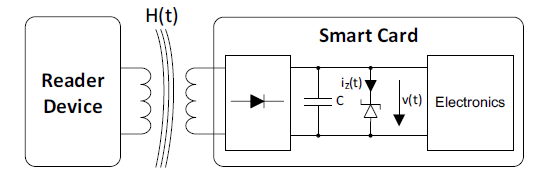
\includegraphics[scale=0.8]{smart_card_internal}
    \caption{Basic internal structure of smart card}
    \label{smart_card}
\label{adhoc}

\end{figure}

Figure \ref{smart_card} shows the basic structure of a smart card. 


\subsection{Machine to Machine(M2M) Communication}
Machine to machine refers to direct communication between devices using any communications channel, including wired and wireless. Machine to machine communication can include industrial instrumentation, enabling a sensor or meter to communicate the data it records (such as temperature, inventory level, etc.) to application software that can use it (for example, adjusting an industrial process based on temperature or placing orders to replenish inventory). Such communication was originally accomplished by having a remote network of machines relay information back to a central hub for analysis, which would then be rerouted into a system like a personal computer. 

\subsection{Security of Smart Cards}
With great advantages smart cards are forced to face some inevitable security issues. Smart card security is associated with both the physical and logical design of the cards. 

\section{Challenges of M2M}
M2M communication system has some major challenges to deal with. Some of the critical challenges are:

\begin{itemize}
\item Terminals may be in hard-to-reach locations (e.g. traffic cameras)
\item Terminals may become geographically dispersed over time (e.g. cargo containers)
\item Owners of large populations of terminals may want to change the network
operator without visiting the terminals (e.g. to change the UICC \footnote{Universal integrated circuit card. For example SIM card})).
\item Terminals need to be protected against unauthorised removal of UICC
\item Terminals may require over-network provisioning after sale or installation.
\end{itemize}

M2M requirements may make the conventional UICC a less advantageous solution for secure authentication. It is necessary to look at the options for a non-personalised security module to which a network operator’s Network Access Application (NAA) can be downloaded. This may be accomplished using an embedded Trusted Environment (TRE) in a terminal. The TRE acts as a hardware root of trust for the storage and execution of secure applications and may also have protected software functions. The TRE may host downloaded software NAAs that emulate the behavior of the USIM  or ISIM  applications.

\section{Challenges of Mobile Networks}
The challenges of M2M intensifies when considered in mobile networks. Mobile networks changes over time and places. The topology changes are too frequent. Data delivery,throughput, bandwidth etc are major concerns in this type of networks. 


\section{Smart Card Security in Mobile Networks}
Current implementation of smart card manufacture has some positive security aspects that plays a great role in using smart card in M2M mobile networks.
\subsection{Physical Tamper-Resistance}
An ISO-7816  smart card has, in practice, a single-chip architecture with little possibility of monitoring communications between different chips on the card. Smart card ICs are designed and implemented to prevent probing and reverse-engineering. They are fabricated on a dedicated production line in a secure facility. Measures include scrambling of busses and of memory addresses, bonded passivation layers, permanently disabled test points, self-generated programming voltage.

\subsection{Proprietary, Secure O/S}
The Smart card’s standardised API, e.g. [4], consists of a restricted command set that has no hidden commands or access methods. It is trusted because of its own built-in security mechanisms and because of those of the underlying hardware platform. It is non-updateable. \newline For applications such as USIM, the Ki and OTA keys are stored and accessed by the O/S in proprietary ways. The O/S cannot be made to reveal the values or memory locations of those data. Conventional GSM SIM cards did not allow adding applications to a live card. The advent of the Javacard now allows applications on a multi-application UICC platform to be updated, deleted or added to an issued card, either remotely or locally. The potential of Javacard for Network Operators is currently restricted by:
\begin{itemize}
\item Implementation by Network Operators of only SMS as the bearer (for OTA messages to the UICC), which has a very limited bandwidth 
\item OTA security standards [11] are not profiled for IP bearers 
\item Lack of a sufficiently rich terminal/UICC interface on nearly all MEs \footnote{A few terminals have implemented the JSR177  terminal/UICC interface, but it’s usually only the SIM toolkit part and not the general APDU API. A few Windows Mobile MEs have allowed an open APDU API to the UICC, using the terminal’s RIL (Radio Interface Layer) but it is not clear if those are still in production}
\item General concerns about the security of multi-application Javacards.
\end{itemize}
In the world of telecoms, it is generally up to the buyer to perform a due diligence test on the smart card vendor to ensure that the O/S has been properly developed and evaluated.

\subsection{Other Measures}
Smart cards include proprietary measures to prevent attacks such as slowing down the external clock and measures against power analysis attacks by the use of noise-free computational algorithms and/or injection of artificial noise and/or damping of noise on the power rail. There are also said to be a large number of detailed precautionary measures taken, some of which are described in the public domain.
\subsubsection{Design and Development Process}
Security is designed into a smart card IC in the secure facilities of a semiconductor manufacturer. The computers that are used for this are isolated from the rest of the world. Undocumented counter-measures in the IC are supported by corresponding design criteria. Once the O/S development is finished, the entire source code may be checked by an independent evaluation.
\subsubsection{Supply Chain}
There are only a handful of world-class vendors of smart cards, so it is feasible for Network Operators to perform the necessary security audits. There will be an agreed arrangement for transferring the Ki objects between network operators and UICC vendors. Ki values cannot be retained in the vendors’ personalisation systems or be discovered by system operatives.

\subsubsection{Security Evaluations}
Card vendors have their O/S independently evaluated and MNOs perform security evaluations of their card vendors’ products and facilities. GSMA [15] provides non-public guidance to its members on how to do that. Common Criteria Protection Profiles have been published for smart cards. One of these [16] is aimed at the underlying IC platform but some are aimed at payment cards issued by financial institutions such as Visa and Mastercard. Cost can be an issue for wider adoption of these evaluation regimes. There are no standard specifications or protection profiles for the security evaluation of telecoms smart cards such as UICCs.

\subsubsection{Terminal Interface Security}
The UICC employs some security measures in the interface with the terminal:
\begin{itemize}
\item User Authentication: PINs (called CHV1 and CHV2 in a SIM card), provide some level of protection with user authorisation on the interface. CHV1 can be disabled by the user, in which case there is no PIN-protection for making calls. The use of CHV1 and CHV2 poses a security vulnerability since the passwords get transported across the UICC-ME interface in clear. The UICC does not authenticate itself to the user, although 3G authentication  provides mutual authentication of the card and the network. In M2M, a remote user could rely on two possible methods of assuring himself of the authenticity of a UICC, i.e. (a) using a remote access protocol that exploits a pre-shared or private key on the UICC and/or (b) using e.g. Liberty Alliance  protocols to trigger the UICC issuer to perform an authentication of the UICC and possibly binding that to the remote access session.

\item  Commands to the UICC are not secured unless they are inside a 3GPP OTA envelope . That is why ETSI and 3GPP have recently specified secure channels and their key establishment methods across the terminal-UICC interface. ISO 7816 and EN726  define secure messaging between a terminal and a smart card but key distribution was not defined (it being assumed that it would be based on pre-installed keys). ISO7816 also defines a set of security-related commands. Neither the ISO nor CEN techniques are included in UICC specifications such as ETSI and 3GPP secure channel specs and compliment the ISO and CEN standards by defining methods for key distribution between the terminal and UICC. There does not seem to be any reason to believe that normal terminals can be trusted to store the distributed key. Protocols such as Global Platform, ETSI RAM/RFM and 3GPP OTA provide end-to-end security from server to card for the purpose of loading and managing files and applications on the UICC. They do not require a secure ME/UICC interface\footnote{Remote Application Management can theoretically be used to download any Javacard application to a UICC and to store it in a security domain. It does not currently apply to the U(I)SIM applications, as there is no standardised mechanism for the UICC to extract and store the Ki and algorithm customisation parameters. For the case of updating existing files either locally or remotely, this is possible only where the access conditions in the File Control Parameters can be satisfied. Remote (OTA) file update is possible on files in any application on the UICC, but only if the files were OTA-enabled at the time the file was created on the UICC}.

\item Protection of data across the interface: All standardised command-sets of a UICC are designed to be sent in the clear across the terminal/UICC interface. Protocols that may be subject to replay attacks must have counter-measures built in, e.g. the sequence numbers used in 3G authentication. In future, the Smart Card Web Server (SCWS), could use HTTPS/TLS to establish a secure tunnel from card to server (or to terminal) via which usernames and passwords could be sent.

\item Access control: In general, access control lists (ACLs) are not used in today’s UICC O/Ss. Access to file operations relies on the principle that if the entity accessing the file can satisfy the access policy (embodied in the File Control Parameters), then it must be an authorised entity.
\end{itemize}



\section{Meeting M2M Requirements with Smart Cards}
Followings are the features of smart card that make it a suitable candidate to use in M2M mobile networks.
\subsection{Advent of the "Big SIM" UICC}
Recent innovations in smart card technology could go a long way to enabling the UICC to fulfill the M2M requirements. The new features described below, plus the ability to store downloaded applications and multimedia files, would need the large memory of "Big SIM". 

\subsection{Large Memory}
Recently, Smart cards with flash memory of up to 2Gbytes have become available.

\subsection{High-Speed I/O}
The conventional I/O speed of the UICC or terminal interface is only a half-duplex 9.6Kbit. In order to be able to move data on and off the Big SIM in a meaningful timeframe is required. Modern smart cards can be equipped with this speed.


\subsection{Smart Card Web Server (SCWS)}
The advent of Mega SIM with USB I/O enables the UICC to support an IP stack and web server. There are a number of advantages to this, e.g. use of (X)HTML to communicate with the UICC. UICCs could even have their own IP addresses, which could introduce a whole set of security issues. ETSI SCP has standardised SCWS and IP on a UICC. Use of SMS for application download is limited in practice to about a 1kByte payload, i.e. 7 concatenated SMSs. Even then, this requires a dedicated SMS-C to achieve an effective success-rate. With ordinary SMS-Cs whose resources are shared with mainstream SMS, the practical limit may be as little as 2 concatenated SMSs, i.e. about 300 bytes. The size of a download using an IP bearer does not suffer from such limitations.

\subsection{Internal Security Domains}
Global Platform has specifications that define security domains on a Javacard smart card. ETSI SCP are now expanding upon these in their specifications for "Confidential Applications." This allows the card issuer to set up domains for the use of third parties to load applets onto the card. The issuer cannot examine those applets. The UICC provides a sandbox environment in which the domains are isolated from each other – a feature that has been somewhat limited in Javacard implementations up to now.

\section{Some Example of usages of Smart card in M2M mobile networks}
\subsection{Smart Cards in the Public Transport Industry}
The advantages of utilising smart card technology,
more importantly contactless smart cards, in the
transport industry have long been realised.\cite{ref4} Some key motivations for smart card based transport industry includes:
\begin{itemize}
\item Low Cost Smart/Chip Card Technology
\item Contactless Smart Card Technology
\item Fraud detection and prevention
\item Easy and flexible transportation
\end{itemize}

Some of the practical examples of smart card usages in public transport are:
\begin{itemize}
\item Oyster Smartcards in the London Underground Subway System (started in 2005)
\item Travel smartcard for students in Australia(started in 2007)

\end{itemize}
In Asia countries like China,Singapore are also using smart card base public transport system in some sectors.

\subsection{Smart Cards in Healthcare Information Systems}
Healthcare Information Services (HIS) have great
potential to enhance the services offered by the
healthcare industry, towards increasing productivity,
lowering costs, reducing medication errors, increasing
transparency and fraud detection and easing the manpower
shortage in healthcare.\cite{ref_2}
Some examples of smart card based healthcare system are:
\subsubsection{Gesundheitskarte}
Started in Germany in 2006. Data in the smart card includes e-Prescription,
Health insurance
Voluntarily:
Medical treatment
history, Emergency
datab. Smart cards are used for e-Prescribing
Insurance
check,
Medication
Log, EHR,
e-Referral.

\subsubsection{Carte Vitale}
Started in 1998 at first then in 2007 new project was launched named Carte Vitale 2 in France. Smart card data includes Informationala,
Health insurance
Emergency datab
Medication for
chronic diseases
Emergency Contact
information. Smart cards are used for e-Prescribing
Insurance
check,
EHR. Figure \ref{smart_card_france} is the first smart of Carte Vitale project.

\begin{figure}[!t]
\centering
    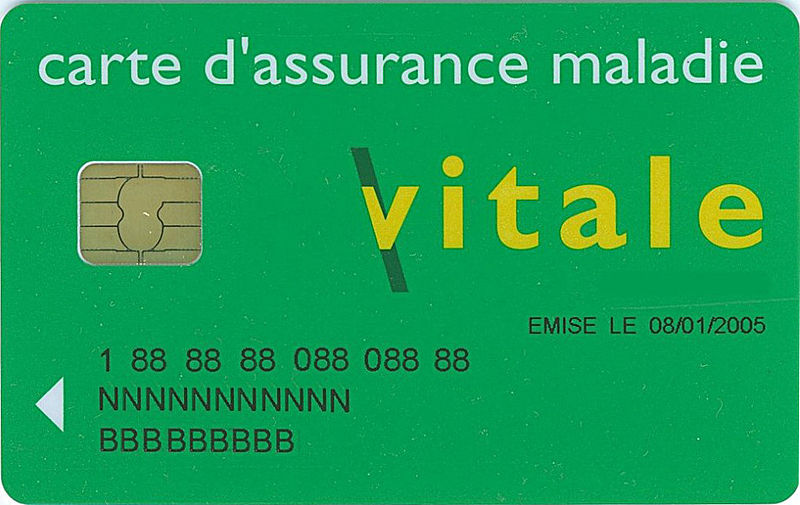
\includegraphics[scale=0.3]{smart_card}
    \caption{An example of a smart card: The Carte Vitale used for health
insurance purposes in France}
    \label{smart_card_france}
\label{adhoc}

\end{figure}


\section{Limitations and Challenges of Smart card in M2M Mass Communication Market}
Despite the many benefits and opportunities that result
from the use of smart cards in M2M mobile networks, smart
cards haven’t taken over as the default technology in
healthcare data management due to several limitations
related with their use.


\subsection{Attacks Against Smart Card Component}
There are two types of non volatile memory in a
smart card. The Read Only Memory (ROM) hold’s
persistent information (e.g. the smart card operating
system, applications), which is written (masked) during
the manufacturing phase. The most common type of
memory that allows information to be written or
deleted at any point in the cards lifecycle is the
Electrically Erasable Programmable Read Only
Memory (EEPROM). Therefore, the target of an
attack can be the security sensitive information stored
internally within the card. The aim of the attack will
be to obtain access to such information and use it to
compromise the security of the card or some other
principal entity in the smart card scheme. \newline
There are two types of non volatile memory in a
smart card. The Read Only Memory (ROM) hold’s
persistent information (e.g. the smart card operating
system, applications), which is written (masked) during
the manufacturing phase. The most common type of
memory that allows information to be written or
deleted at any point in the cards lifecycle is the
Electrically Erasable Programmable Read Only
Memory (EEPROM). Therefore, the target of an
attack can be the security sensitive information stored
internally within the card. The aim of the attack will
be to obtain access to such information and use it to
compromise the security of the card or some other
principal entity in the smart card scheme.
A smart card attack can also target the operation of
cryptographic primitives (e.g. the generation of
cryptographic keys or execution of an application) of
the actual smart card microprocessor. The aim of this
attack will be to force the smart card microprocessor to
perform certain operations that will compromise its
security. For example, to allow the microprocessor to
update the ticket entitlement in the card and at the
same time avoid deducting the payable amount from
the purse. The range of attacks on smart cards can be
classified into three basic categories i.e. logical,
physical and side-channel.

\subsubsection{Logical attacks}
The logical types of attacks attempt to identify and
exploit any vulnerabilities or weaknesses in the design
of the smart card operating system (SCOS) or
the smart card application. This may take the form of
presenting the card with invalid commands, formats,
field lengths or attempts to overflow buffers. The
advantage of these attacks is that they are cheap,
relatively simple to perform and do not necessarily
damage the card. However, provided that reputable
application developers and smart card suppliers are
used then rigorous design (and sometime peer reviews)
and development processes should have eliminated the
logical vulnerabilities.

\subsubsection{Physical attacks}
These types of attacks can be mounted by an entity
obtaining physical access to the smart card. Therefore
the attacker can be either the cardholder, a member of
staff, or even a third party that somehow manages to
get hold of some legitimate cards. \newline
There are many different ways to perform physical
attacks on smart card microprocessors, some require
loaw cost equipment [13] and other require
sophisticated and expensive equipment. Typical
attacks, in the latter category, include attempts to read
the contents of the EEPROM memory of the card (by
using powerful electron microscopes), to re-activate
burned fuses by focusing ion beams or even using laser
cutter microscopes to modify the architecture of the
chip. In most cases a number of chips may have to be
destroyed before an attack is considered successful. In
order to provide adequate countermeasures the smart
card manufacturers provide constant improvements
(Dielectric "passivation layers", wire mesh layers and
non standard bus systems) on their chip designs, in
order to make it more difficult for these attacks to take
place. \newline
Whilst physical attacks have focused on smart cards
used in other industries there is no reason why they
cannot be applied to transport [4]. The main question is
whether a criminal group can find a business case to
justify the cost and effort required for such an attack.




\subsubsection{Side-Channel Attacks}
Side channel attacks have been off concern to the
smart card industry because they require modest levels
of equipment and do not necessarily damage the card.
The majority of attacks have monitored the supply
current of the working smart card in order to infer how
particular processes run and to extract secret
information such as keys stored on the card. Similar
results have been obtained in laboratory conditions by
carefully positioning a tiny antenna over certain areas
of a smart card chip. Attacks can be applied to
normally operating processes or by applying external
input to introduce faults. \newline
There are some industry review of contactless card
security  but up to recently there was relatively
little is said about side-channel attacks on contactless
cards (compared to cards with contacts), primarily
because there was no direct and convenient
measurement of current consumption. However,
current variations may result in detectable RF field
fluctuations which may then be processed. The radio
communication link may also assist the attacker if it
proves possible to locally eavesdrop on normal card
usage.

\subsubsection{Publicity Attacks}
The "publicity" attacks usually come from
researchers and individuals seeking fame and
recognition. Although initially these types of attacks
might not be considered extremely damaging, they
actually are, as they eventually attack the brand image.
In case a smart card application (residing in a multiapplication
smart card) is compromised, it is often the
case that all the accompanying applications receive the
bad publicity. In that case restoring the brand image
can be extremely daunting. For example, suppose a
loyalty point application, an electronic purse
application and a ticketing application are all residing
in the same card. Let us suppose that the loyalty
application is compromised and due to the fact that it is
used alongside the transport application the latter also
receives negative publicity. \newline
The "publicity" attacks can have a devastating
effect both on the actual project and the organisations
involved. The creation of a widely recognized and
successful brand image often requires a huge
investment in time money and effort.

\subsubsection{Indirect Gain Attacks} 
The indirect gain attacks are relatively more
difficult to be identified as they exploit vulnerabilities
in various components of the system and they are
usually identified following the system being fully
operational. For example, an attacker exploits
vulnerabilities in the protocol or the messages being
exchanged to/from the smart card.
\subsubsection{Attacks by Rogue Terminals}
This is the classical type of attack that alarmed both
cardholders and card issuers in the past [3]. Whenever
a smart card is presented to a legitimate terminal, the
terminal should be trusted that it will perform all the
operations as expected. For example, consider the case
of a cardholder buying a ticket from an unattended
POS terminal in the street. The cardholder is prompted
to pay £1 for the ticket price but the terminal deducts
more (e.g. £5) from the purse. It is likely that the
rogue transaction will be identified when the backoffice
systems or the cardholder inspects the card log
files or the card transaction statements/receipts
respectively, but this may be too late to take effective
action.


\subsubsection{Attacks Against the Terminal and/or
Interface}
For terminals that reside under the cardholder’s
control (e.g. a PC connected reader) there is always the
risk that the communication might be intercepted
and/or manipulated. However, if the communication
protocol and the applications are properly designed and
communication is adequately protected (e.g. encrypted
or signed) the likelihood and the effects of an attack
are minimised.\newline
Irrespectively of the terminal characteristics or the
relevant cardholder control, there is the risk of the card
being removed from the terminal before the transaction
is completed. The duration of a typical contactless
transaction in a transport application may be between
140-300ms. This means that the time frame, that an
attack can be mounted, is relatively small. In cases
where the terminal is not under the immediate control
of the cardholder (e.g. entry gates or POS) it becomes
even more difficult to control the timing of such an
attack. Moreover, most of the cards provide the
functionality of transaction atomicity. This means
that well designed applications will guarantee that
transactions will either take place in full or do not take
place at all.

\subsection{Non-technical Challenges}
\begin{itemize}
\item Cost: One of the main limitations is the cost of replacing the
existing infrastructure, with smart card. 
\item Data management: Management and proper monitoring of collected data is a major challenge. Lack of proper equipment and manpower could hamper the whole system.
\ Public reaction and new technologies: An obstacle that must be overcome is some involved
parties reactions to the implementation of a smart card.
The technical training needed to operate it, the system's high
complexity and security concerns.

\end{itemize}

\section{Known Attacks Against Smartcards}
Smart Card technology had experienced some crises in the past, as follows:
\subsection{Side Channel Attacks (specifically Power Analysis)}
This type of attack relies on the noise on the smart card’s power contact being correlate-able with the processing that is going on in the UICC, especially when it is reading the values of a secret key into its internal registers. This can work well on an unprotected card that uses the DES algorithm. RSA is not susceptible and neither is AES (upon which 3GPP Milenage is based).\footnote{This attack was successfully perpetrated against the pilot of a well publicised smart card payment system in the UK. Although the scheme was designed to use RSA with unique private keys, the pilot used DES with a global key on every card.} It is easy to prevent this type of attack at the design stage of a smart card. The physical structure of an embedded TRE would be such that it would not leak this information. There would be no such interface that an attacker could monitor and the processing in the TRE would be such that any noise occurring on any power rail would not contain any recoverable information.
\subsection{Probing of Broadcast TV Cards}
Satellite TV smart cards have to contain global decryption keys, due to the nature of the service, i.e. a broadcast encrypted signal. If you crack one card, you have cracked the whole scheme. This is, of course, not true of networked telecoms systems.

\subsection{Cloning of SIM cards}
The only verifiable instance of cloning of 2G SIM cards was a "known plaintext" (50,000 challenge-response pairs) attack against the COMP128 authentication algorithm and not against the card platform itself. This attack has been prevented by the use of better algorithms and is not at all possible with 3G. The relevance of this attack to TREs is that it has gone down in the annals of urban mythology as an attack on the SIM card, rather than an attack on the algorithm. "Mud sticks", as they say.
\subsection{Others}
Some other known smart card attacks include:
\begin{itemize}
\item Attacks Against Disposable "Eurochip" Phonecards
\item Timing Attack on RC5 \cite{timing_attack}
\item EEPROM Alteration by BUS probing \cite{probing_attack}
\item Depackaging \cite{probing_attack}
\end{itemize}


\section{Enhancements Required for M2M Mass Market}
A Smart card to be used in mass-market M2M applications would have to support the requirements of long life-time with long maintenance intervals, non-removability, remote download of operator’s authentication application and remote change of operator. Some very significant enhancements need to be considered as follows:

\subsection{Security Domains}
Support is required for security domains for the card issuer and for third parties, e.g. as per the SCP specifications "Confidential Applications" concept. But in the M2M scenario, network operators would be classed as third parties. In order for the card issuer to allow the M2M equipment owner to change to a new network operator, the card issuer (who is therefore not a network operator) assigns a domain to a new network operator and closes the domain of the old network operator.

\subsection{Removable UICC vs. Downloadable UICC}
Unauthorised removal of a traditional "removable" UICC must be made very difficult, while its replacement must be easy. A better alternative to this is to fix the UICC in the terminal and for it to support the ability to download MIDs. Such a UICC must be able to extract Ki objects and similarly sensitive data from messages from a remote server and lock them away in secure memory so that they cannot be revealed to entities outside the UICC. Network operators will demand that there be no reduction of security in UICCs that support these features.

\subsection{Secure Download Protocols}
Support is required for secure download protocols other than standardised OTA, i.e. M2M requires protocols which do not require pre-shared keys and which can be used over IP bearers. (In this respect, support for SCWS and IP stack could be an advantage).


\subsubsection{Options for Secure Downloadable Identity} 
Option for client-side authentication technologies for M2M could include:
\begin{itemize}
\item UICC with download capability
\item An embedded TRE in the terminal, to provide a secure execution and storage
environment. Authentication applications (Managed Identities or "MIDs")
would be downloaded to the TRE over public IP networks.
\item Smart token such as the new multimedia card with on-card UICC (or SMC)

\end{itemize}

A framework of standardised specifications is needed for the above solutions. The discussion within standardization about the (dis-)advantages of the various candidate solutions is lively and far from concluded. A TRE(Trusted Environment) based solution is proposed. Figure \ref{tre} shows the proposed structure.

\begin{figure}[!t]
\centering
    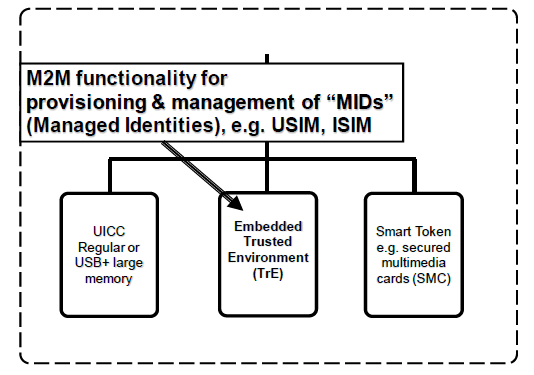
\includegraphics[scale=0.8]{tre}
    \caption{Options for Secure Environments for Downloaded Identity Credentials}
    \label{tre}
\label{adhoc}

\end{figure}

\begin{table}[]
\centering

\begin{tabular}{|L{4cm}|L{4cm}|L{2cm}|L{2cm}|}
\hline
\textbf{Required Feature} & \textbf{UICC \cite{uicc}} & \textbf{TRE} & \textbf{SMC \cite{smc}} \\ \hline
Currently standardised & good & medium (it could be based partly on TCG specs) & medium \\ \hline
Currently available & good & medium (some limited versions available) & poor \\ \hline
Protection against unauthorised removal & poor (good, if M2M form factor UICC is soldered in) & good & poor \\ \hline
Provides secure API & good & good & not known \\ \hline
Does not require connector and interface chips & poor & good & poor \\ \hline
MIDs can be downloaded & poor. Can’t download NAAs & good & poor. Can’t download NAAs \\ \hline
Key management suits M2M model & poor (pre-shared keys for authentication and download) & good (can use PKI) & poor \\ \hline
Predictable costs & poor (for full-function, big memory, downloadable UICC) & Good (part of chipset) & poor \\ \hline
Secure channel to terminal & poor (standardised but usually not implemented) & good & not known \\ \hline
Remote change of operator & poor & good & poor \\ \hline
Open API for download & poor & good & poor \\ \hline

\end{tabular}%

\caption{Comparison of Solutions for Secure Downloadable Identity}
\label{comparison}
\end{table}
Table ~\ref{comparison} shows the comparison between different options.
No solution comes out as perfect, but the TRE shows promise if it can be standardised. The UICC shows promise if its current limitations (including that of lack of implementation of already-standardised features in cards and terminals) can be overcome

\subsection{Secure Interface to Terminal}
Support for a secure terminal-UICC interface may be a requirement, as discussed above.

\subsection{Smart Card Distribution and Storage}
Smart Card Distribution and Storage should
always be considered as a sensitive process. Especially
within the transport industry where smart cards will
have to be transported pre-personalised within various
sites, e.g. from the manufacturer to the issuer and from
the issuer to the various storage locations at the various
points of sale. Therefore, card transportation and
distribution should always take place via approved
couriers.
Furthermore, if the keys used for card enablement (e.g.
in order to protect the cards during their transportation
through various sites) remain secret then the cards will
remain relatively secure.

\subsection{Smart Card Destruction and Replacement}
It must be guaranteed that the
selected cards are properly disposed of and furthermore
any residual value within the electronic purses is
properly reclaimed. The monetary refunds procedures
should be adequate in order to prevent staff from
exploiting residual value stored in lost or non working
cards, or even attackers picking old cards and creating
disposal clones.


\section{Future Works}
Our future work concerns the integration of fault effect
analysis into our reader/smart card system exploration framework in M2M.
This is accomplished by adding emulation-based fault
injection techniques. Thus, faults affecting the reader's or the
smart card's functionality, performance, power consumption,
and power supply can be evaluated early during the design
phase.


\section{Conclusion}
From a technology point of view all the components
that assist the deployment of smart cards in the
M2M mobile networks are available. Selecting the best
available technology will probably reduce certain risks
but at the same time will increase the overall cost of a
migration program. Furthermore, the proper system
integration, installation and operation should be
considered as critical phases.
\newline
Smart cards tend to be replaced every 2-3 years, in order to catch up with
recent technological developments. Selecting the
appropriate smart card technology is a very critical step
for the transport operator as the appropriate balance
between price and offered technology should be
identified. Similarly, there are other issues (backoffice
systems, station gating, POS terminals, third
party applications, etc.) that will have to be considered
for an effective chip migration. With proper installation and system architecture smart card in M2M mobile systems, can serve a long way to facilitate us.


\newpage
\begin{thebibliography}{9}

\bibitem{main_paper}
\textbf{Security Aspects of Smart Cards in Machine-to-Machine (M2M) Advanced Mobile Network Applications.}
Mike Meyerstein1, Inhyok Cha, Yogendra Shah

\bibitem{ref_2}
Smart Cards in Healthcare Information Systems: Benefits and
Limitations
Anastasis P. Keliris, Vassileios D. Kolias and Konstantina S. Nikita.IEEE Veh. Technol. Mag., vol. 8, pp. 24-30, Mar. 2014
\bibitem{ref3}
H. Cripps, C. Standing and V. Prijatelj, "Smart health care cards: Are
they applicable in the Australian context?", presented at the 25th Bled
eConference,2012

\bibitem{ref4}
Overview of Security Threats for Smart Cards in the Public Transport
Industry.Konstantinos Markantonakis, Keith Mayes,Konstantinos Markantonakis, Keith Mayes,Konstantinos Markantonakis, Keith Mayes

\bibitem{timing_attack}
A Timing Attack on RC5, By Helena Handschuh and Howard M. Heys

\bibitem{probing_attack}
Probing Attacks on Tamper-Resistant Devices, By Helena Handschuh, Pascal
Paillier and Jacques Stern

\bibitem{java_card}
Java community specification JSR177: Security And Trust Services API
 
\bibitem{iso_1}
ISO/IEC 7816-1, "Identification cards – Integrated circuit(s)
cards with contacts" 

\bibitem{uicc}
3GPP TS 31.102; Characteristics of the USIM Application
3 3GPP
\bibitem{smc}
3GPP TS 31.103; Characteristics of the ISIM Application
\bibitem{esmi}
ETSI TS 102 221: UICC-Terminal interface; Physical and logical characteristics

\bibitem{fina_ref}
S. Mangard M. Hutter and Martin M. Feldhofer.
Power and emattacks on passive 13.56 mhz rfid devices. In
Workshop on Cryptographic Hardware and Embedded
Systems, CHES 2007, volume 4727 of LNCS, pages 320–333.
Springer-Verlag, September 2007.

\end{thebibliography}





\end{document}
